\documentclass[a4paper,11pt]{article}
\usepackage{graphicx}
\usepackage{enumerate}
\usepackage[usenames, dvipsnames]{color}
\usepackage[margin=1.25in]{geometry}

\begin{document}

\begin{flushright}

\vspace{1.1cm}

{\bf\Huge Project 3}

\rule{0.25\linewidth}{0.5pt}

\vspace{0.5cm}
%Put Authors
Justin Ely
\linebreak
\newline
%Put Author's affiliations
\footnotesize{605.462 Data Visualization \\}
\vspace{0.5cm}
% Date here below
07 March, 2017
\end{flushright}

\noindent\rule{\linewidth}{1.0pt}

%%%%%%%%%%%%%%%%%%%%%%%%%%%%%%%%%%%%%%%%%%%%%%%%%%%%%%%%%%

\section{Data}
The dataset chosen for this project comes from the Baltimore open data portal.  It contains, excluding juvenile bookings, the arrest records processed at Baltimore's Central Booking and Intake Facility.  The dataset is provided by the Baltimore Police Department, updated monthly, and maintained by Jeffry Cooper.  It can be found at the following url: https://data.baltimorecity.gov/Public-Safety/BPD-Arrests/3i3v-ibrt.

This dataset has 138,000 records and 15 columns.  Each record is an individual arrest with associated information about the crime.  A description of each is given in the table below.

\begin{center}
\begin{tabular}{| l | l | l | }
  \hline	
      Variable & Type & Description  \\  \hline \hline
      Arrest & ordinal numeric & Unique arrest ID \\ \hline
      Age & ordinal numeric & Age of the offender \\ \hline
      Sex & categorical nominal & Gender of the offender \\ \hline
      Race & categorical nominal & Race of the offender \\ \hline
      ArrestDate & quantitative interval & Date of the arrest \\ \hline
      ArrestTime & quantitative interval & Time of the arrest \\ \hline
      ArrestLocation & arbitrary nominal & Address the arrest took place \\ \hline
      IncidentOffense & arbitrary nominal & Description of the reason for arrest \\ \hline
      IncidentLocation & arbitrary nominal & Address the arrest took place (duplicate)\\ \hline
      Charge & ordinal numeric & Code for the charge of the arrest\\ \hline
      ChargeDescription & arbitrary nominal & Description of the charge for the arrest \\ \hline
      District & categorical nominal & Region of the incident\\ \hline
      Post & ordinal numeric & ID of the police post\\ \hline
      Neighborhood & arbitrary nominal & General neighborhood of the incident \\ \hline
      Location & quantitative interval & Geographic latitude and longitude of the incident \\ \hline
\end{tabular} \\
\end{center}

\section{Possible Questions}
This dataset makes possible a number of avenues of investigation.  Stats on police arrests can be used to probe the behavior of the officers, the commonality of certain types of crimes, and trends across time to name just a few.  Just a few questions that could be asked are listed below. 

\begin{enumerate}
  \item What time of day do most arrests happen?
  \item How has the number of arrests changed year-to-year?
  \item Does age, sex, or race have a correlation with number of arrests?
  \item How are the arrests distributed across Baltimore?
  \item What charges are most common?
\end{enumerate}

\section{Dashboard}

\begin{figure}[h!]
\caption{Dashboard to analyze the Baltimore City arrest data.} 
\centering
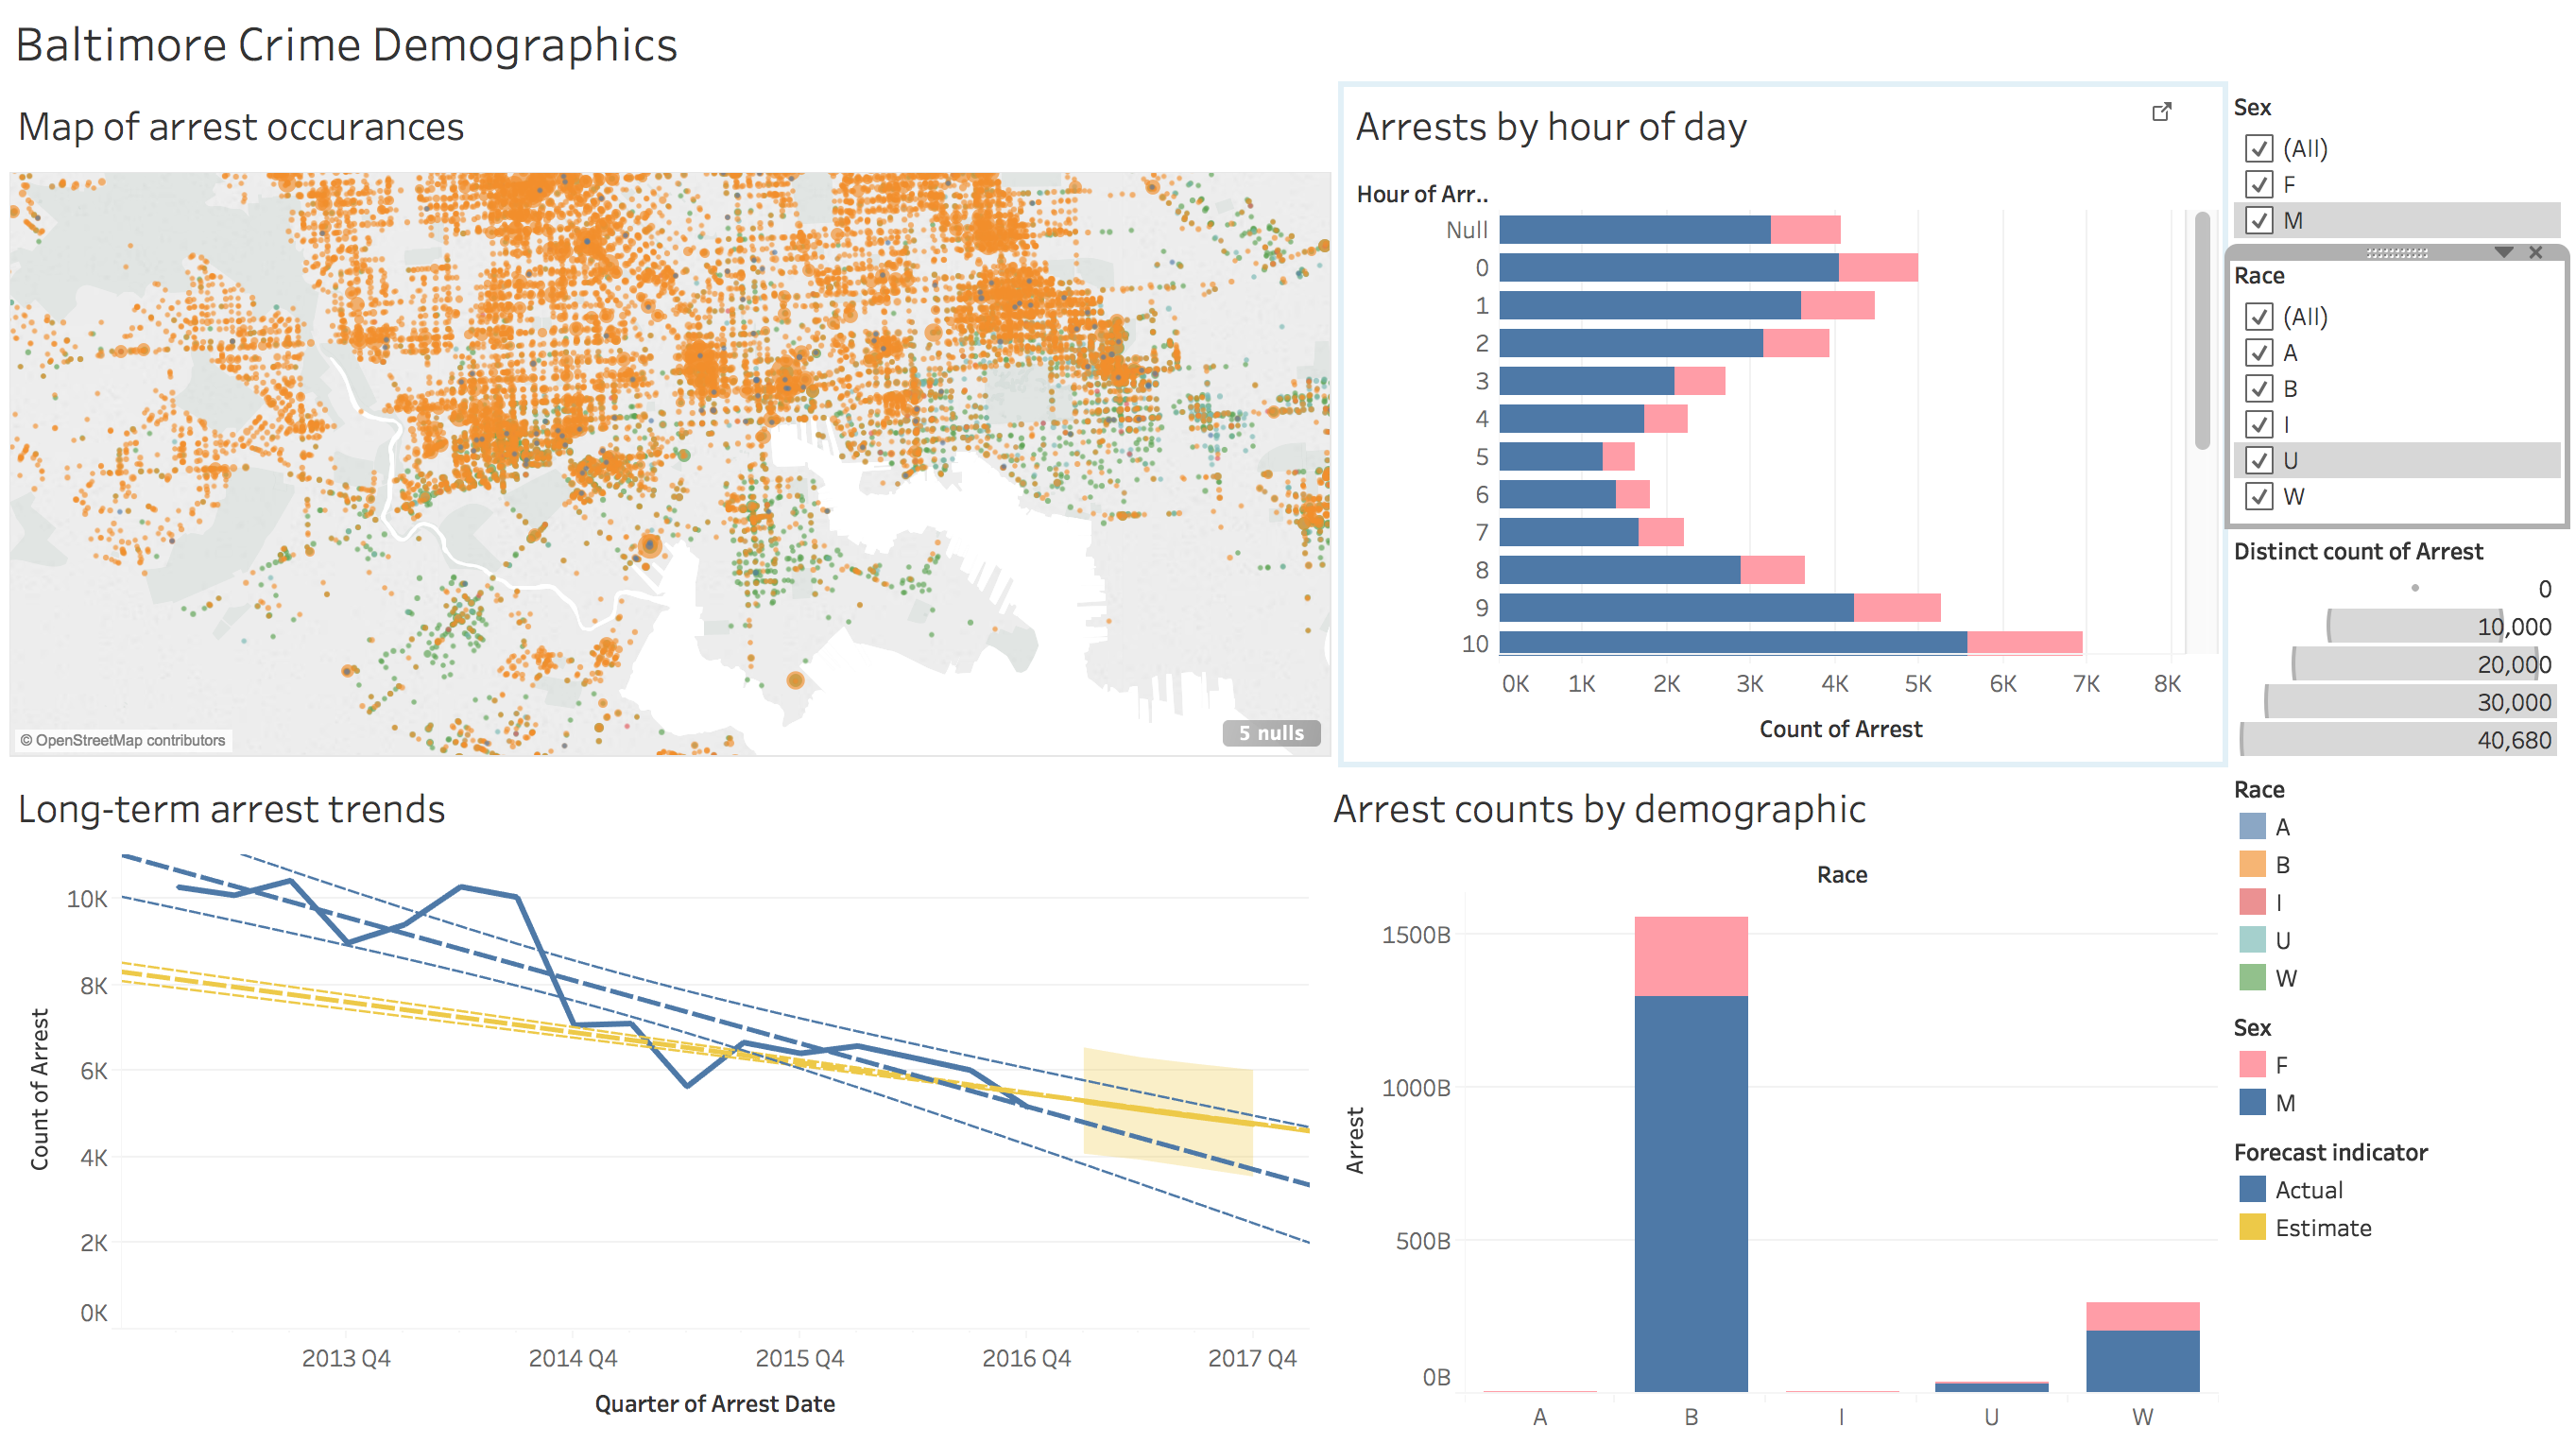
\includegraphics[width=.8\textwidth]{dashboard.png}
\end{figure}

The dashboard combines four individual views into one single tool.  The top-left plot is a map showing the distribution of arrests across the city.  Each mark is color-coded to the race of the arrested individual, and is sized according to the number of arrests that happened in that location.  The top right is a bar-chart showing the number of arrests that have occurred during each hour of the day.  A line chart showing the total arrest count across time is shown in the bottom left.  This plot contains a linear fit and an extrapolated prediction from the data.  The last chart, shown in the bottom right, is a bar chart showing the arrest count for each race.  Each chart can be filtered by race and gender, and the two bar-charts display male and female records by the well-understood colors of pink and blue, respectively.  

The dashboard was created with the purpose of facilitating the understanding of the reported Baltimore crime data.  More than 138k records, each with 15 different characteristics, is impossible to understand from a simple table view.  Instead, the dashboard brings forward pertinent information in an easily accessible way.  This view lets viewers quickly gain an understanding of the geographic, time, and demographic breakdown of arrests in Baltimore City.  By filtering on gender and race, they can refine the massive dataset and view trends or outliers in subsets of the population.

Though this data may permit many other studies, like studying the incident description, many of these free-form columns were too irregular to incorporate into the dashboard as-is.  Significant cleaning would have to be done before reading in the data to gain significant insight into many of these interesting columns.

%%%%%%%%%%%%%%%%%%%%%%%%%%%%%%%%%%%%%%%%%%%%%%%%%%%%%%%%%%


\end{document}
